\chapter{Histogram View}
\label{sec:histo_view}

A Histogram View displays the distribution of one numerical variable as a histogram, approximating the statistical distribution of said varable. When started, it presents itself in the following manner.

\begin{figure}[H]
    \hspace*{-2cm}
    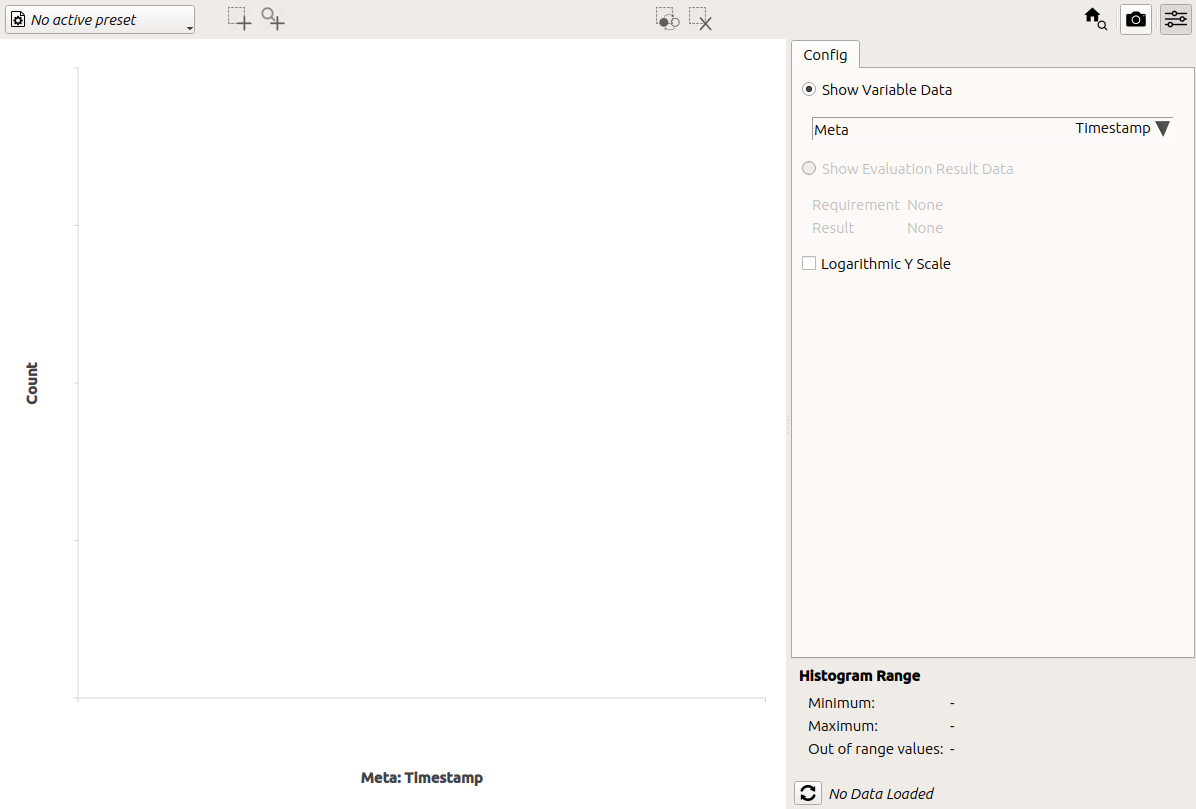
\includegraphics[width=18cm,frame]{figures/histogram_start.png}
  \caption{Histogram View startup}
\end{figure}

\section{Layout}

On the left side resides the plot area in which the histogram is shown (if data has been loaded). 
The tool bar at the top shows the currently selected tool and the available actions.\\

On the right side resides the configuration area, which allows configuring what data is loaded and how it is displayed.
The 'Reload' button on the bottom can be used to trigger a reload of the view's data.\\

Both areas can be resized and hidden if wanted.

\section{Data Loading}

To load the data the mechanism described in section \nameref{sec:ui_overview} or the 'Reload' button can be used. To filter the dataset, the mechanism described in section \nameref{sec:filters} can be used. \\

\begin{figure}[H]
    \hspace*{-2cm}
    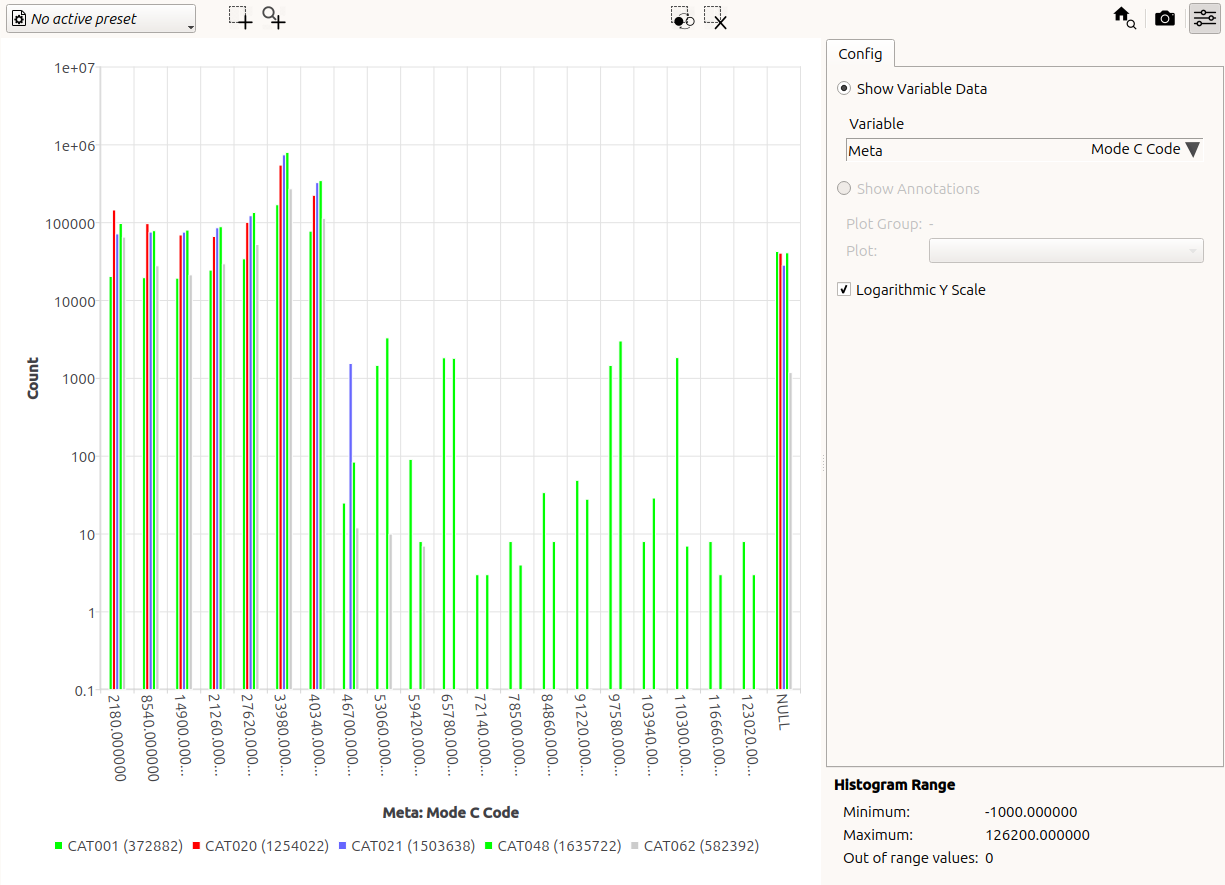
\includegraphics[width=18cm,frame]{figures/histogram_loaded.png}
  \caption{Histogram View after loading}
\end{figure}

On the x-axis the selected variable's data range is discretized into 20 bins. An additional bin represents all NULL values.
%plus one optional NULL value bin), scaled between the minimum and maximum value of the loaded data. 

On the y-axis the bin sizes per DBContent are shown, either in linear or logarithmic scale. \\

Below the histogram a legend is shown, giving the total counts of all data points. \\

% TODO_V7 Per DBContent - correct?
In the current example the meta-variable 'Mode C Code' is used, showing the amount of data present in different flight levels per DBContent.

\section{Usage}

\subsection{Toolbar}

%TODO_V7 Maybe we could reformulate that, as only one button/mode is available after all?
The first button can be used to activate the selection tool (shortcut refers to keyboard shortcut). 

Note that an active tool can always be ended by pressing the 'Escape' key. 

\begin{table}[H]
  \center
  \begin{tabular}{ | l | l | l | l |}
    \hline
    \textbf{Icon} & \textbf{Shortcut} & \textbf{Text} & \textbf{Description} \\ \hline
    \includegraphics[width=0.5cm,frame]{../../data/icons/select_action.png} & S & Select & Allows data selection \& de-selection \\ \hline
    \includegraphics[width=0.5cm,frame]{../../data/icons/zoom_select_action.png} & Z & Zoom & Allows data zooming \\ \hline
  \end{tabular}
  \caption{Toolbar: Available tools}
\end{table}

%TODO_V7 Only refer to keyboard shortcuts when providing them
The others provide general operations.

\begin{table}[H]
  \center
  \begin{tabular}{ | l | l | l | l |}
    \hline
    \textbf{Icon} & \textbf{Shortcut} &\textbf{Text} &  \textbf{Description} \\ \hline
    \includegraphics[width=0.5cm,frame]{../../data/icons/select_invert.png} & & Invert Selection & Selects all de-selected \& vice versa \\ \hline
    \includegraphics[width=0.5cm,frame]{../../data/icons/select_delete.png} & & Delete Selection & De-selects all target reports \\ \hline
    \includegraphics[width=0.5cm,frame]{../../data/icons/zoom_home.png} & Space & Zoom to Home & Resets the current zoom \\ \hline
  \end{tabular}
  \caption{Toolbar: Available operations}
\end{table} 

\subsection{Config Tab}

The elements on the top define which data is visualized in the histogram. \\

Any numerical variable can be visualized by checking the 'Show Variable Data' box and selecting a variable in the selection control below.
A reload operation might be required for the selection to take effect. \\

If available, plottable histogram annotation data of active View Points (e.g. View Points representing evaluation results) can be visualized by checking the 'Show Annotations' box. 
If multiple histogram annotations are present in a View Point, these individual plots can be selected using the 'Plot' combo box.
Plottable annotations might further be grouped into so-called plot groups, which are listed under 'Plot Group'.
The plot group can be switched in case multiple plot groups are available. \\

In the case of evaluation results, the plot group might e.g. display the currently selected requirement result,
the available plots representing different histograms generated by this specific result. \\

\begin{figure}[H]
    \center
    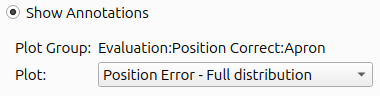
\includegraphics[width=6cm,frame]{figures/histogram_annotation.png}
  \caption{Histogram View showing evaluation results as plottable annotations}
\end{figure}

The 'Logarithmic Y Scale' checkbox can be used to switch between linear and logarithmic scale of the y-axis. \\

\subsection{Histogram}

%\subsubsection{Zoom}

%The mouse wheel can be used to zoom in or out of the presented data. This is in the current presentation only useful in limited circumstances. The space key can be used to reset to the default zoom level (euqivalent to \includegraphics[width=0.5cm,frame]{../../data/icons/zoom_home.png}).

\subsubsection{Selection Tool}
 
If the 'Select' tool is active, data can be selected. Using the left mouse-button a red selection rectangle can be spanned across all bins that should be selected.

\begin{figure}[H]
    \hspace*{-2cm}
    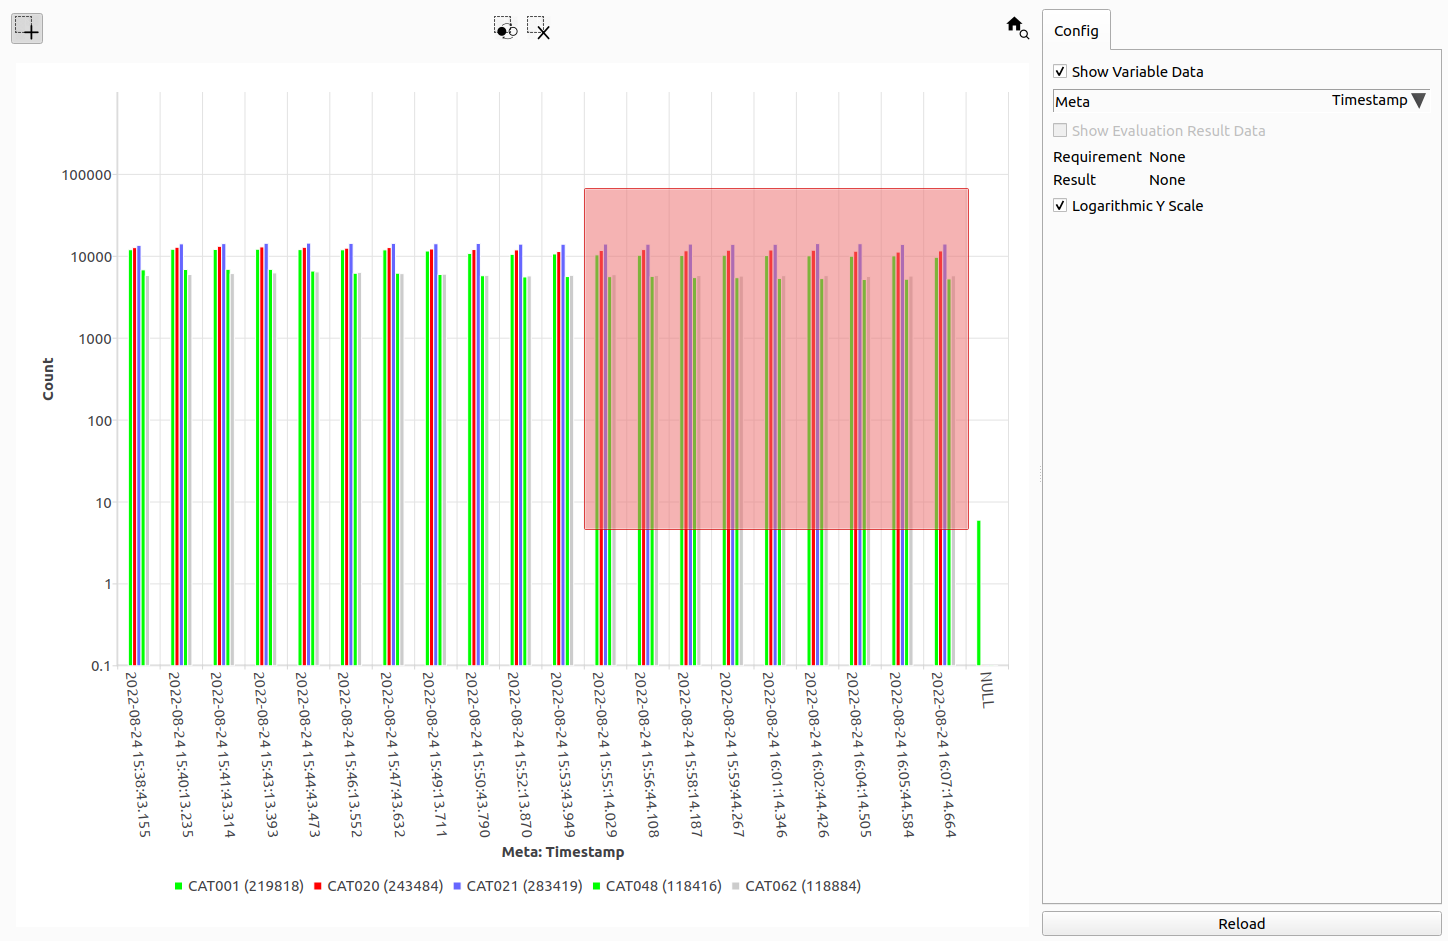
\includegraphics[width=18cm,frame]{figures/histogram_select.png}
  \caption{Histogram View data selection}
\end{figure}

The selected data is then presented in an extra 'Selected' entry in the legend, showing the count of all selected data points.

\begin{figure}[H]
    \hspace*{-2cm}
    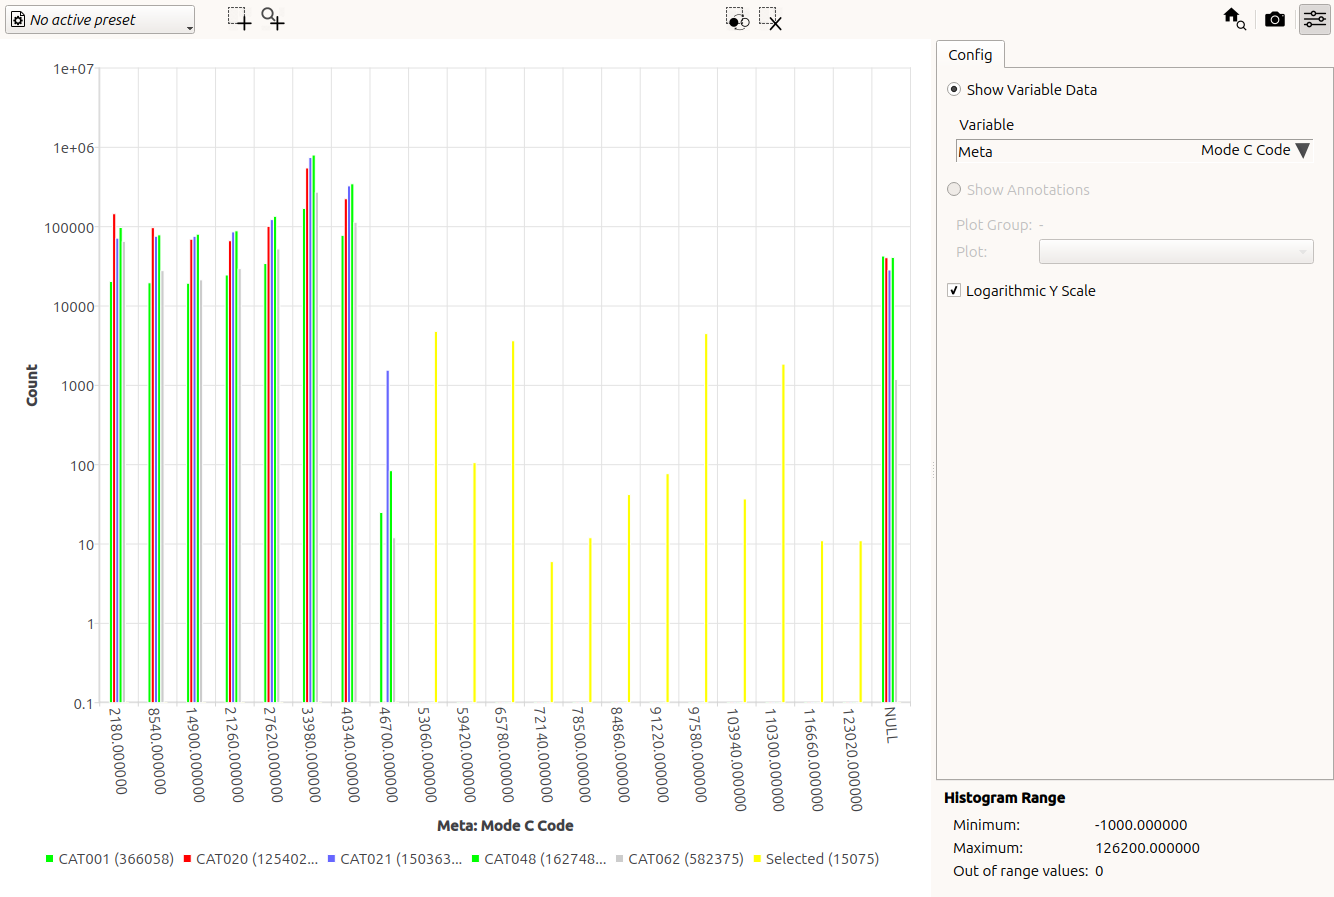
\includegraphics[width=18cm,frame]{figures/histogram_selected.png}
  \caption{Histogram View data selected}
\end{figure}

This enables selection of parts of the data based on the presented variable, allowing deeper analysis e.g. of dubious data. \\

The 'Invert Selection' \includegraphics[width=0.5cm,frame]{../../data/icons/select_invert.png} or 'Delete Selection' \includegraphics[width=0.5cm,frame]{../../data/icons/select_delete.png} actions allow for easier selection of the wanted target reports. \\

By pressing the 'Control' key while selecting, the newly selected data is added to any previous selection. This can be used to select data incrementally, making more complex selections possible.

\subsubsection{Zoom Tool}

The 'Zoom' tool can be used to zoom to a range of bins of the current histogram. Using the left mouse-button a red zoom rectangle can be spanned across the desired region of interest.

\begin{figure}[H]
    \hspace*{-2cm}
    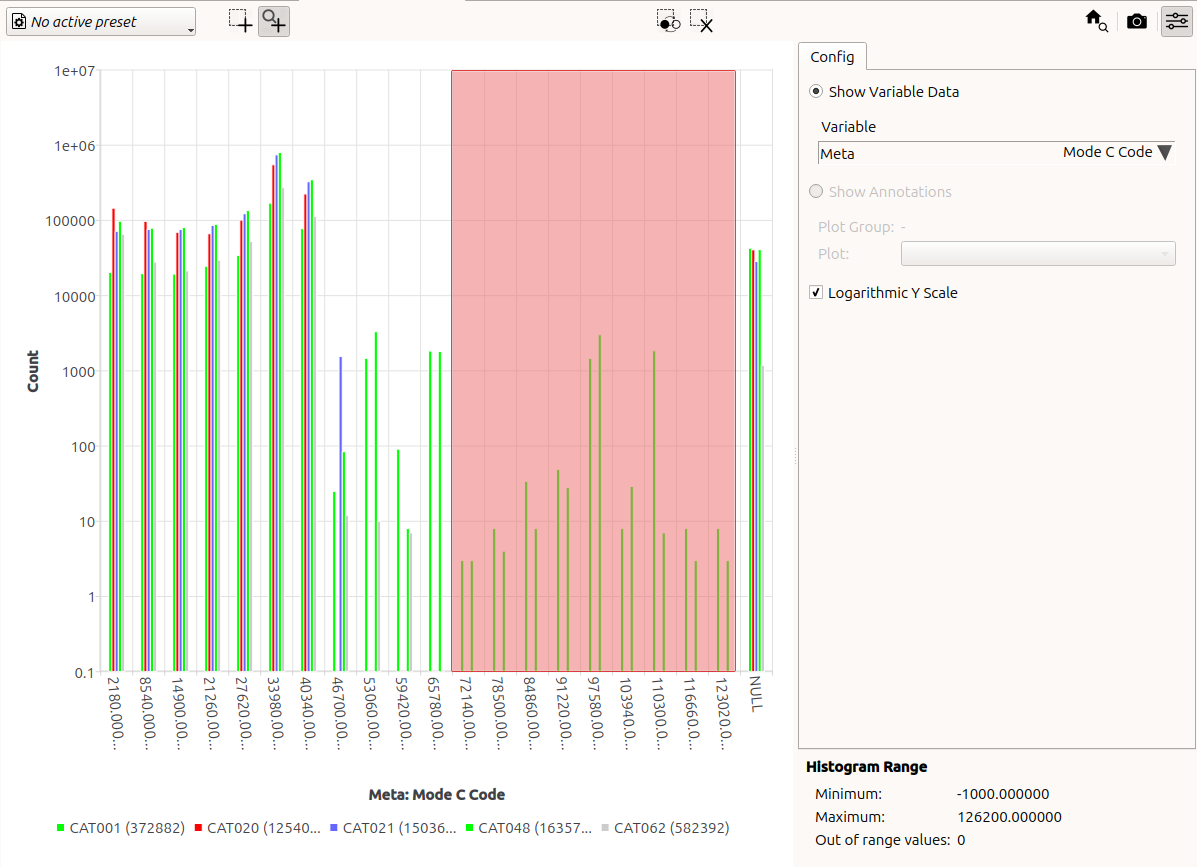
\includegraphics[width=18cm,frame]{figures/histogram_zoom.png}
  \caption{Histogram View zoom selection} 
\end{figure}

A new histogram is generated using the data contained in the selected bins, allowing a closer inspection of the distribution of this data.

\begin{figure}[H]
    \hspace*{-2cm}
    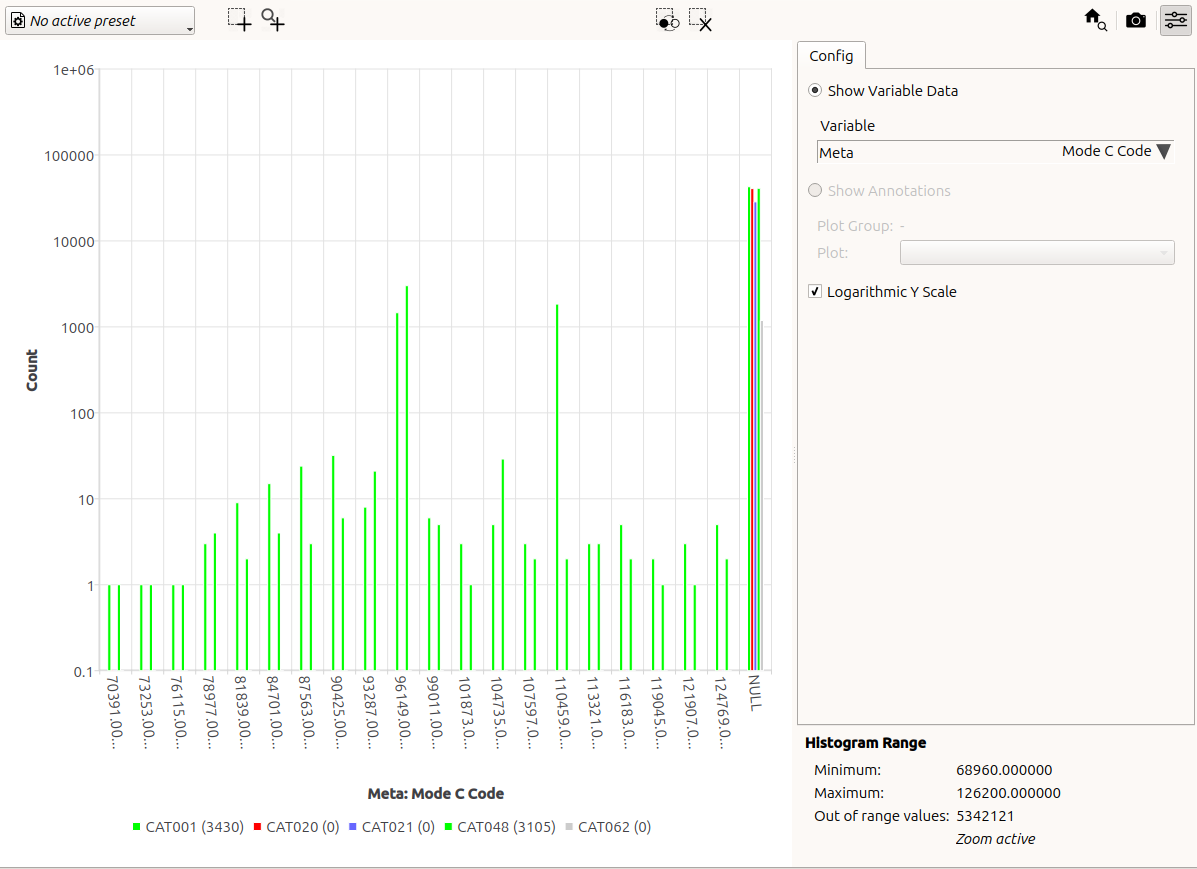
\includegraphics[width=18cm,frame]{figures/histogram_zoomed.png}
  \caption{Histogram View zoom active}
\end{figure}

The histogram can always be reset to the complete data range by pressing \includegraphics[width=0.5cm,frame]{../../data/icons/zoom_home.png} or the 'Space' key. \\

Below the Config Tab the value range of the currently shown histogram is displayed. 
Data items which fall out of this range are counted, this count being displayed under 'Out of range values'.
If a zoom is currently active, this will also show here as '\textit{Zoom active}'.

\begin{figure}[H]
    \center
    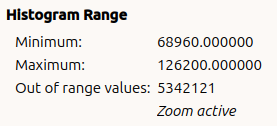
\includegraphics[width=6cm,frame]{figures/histogram_zoom_active.png}
  \caption{Histogram View value range}
\end{figure}

